% ============================================================
%  Systemind Research Technical Report STR-2026-001
%  How Should Your Agent Talk to Mine?
%  Compile with: xelatex (twice)
% ============================================================
\documentclass[10pt,a4paper]{article}

% ---------- Fonts (XeLaTeX) ----------
\usepackage{fontspec}
\setmainfont{texgyrepagella}[
  Path=/usr/local/texlive/2025/texmf-dist/fonts/opentype/public/tex-gyre/,
  Extension=.otf, UprightFont=*-regular, BoldFont=*-bold,
  ItalicFont=*-italic, BoldItalicFont=*-bolditalic]
\setsansfont{Helvetica Neue}
\usepackage{microtype}

% ---------- Layout ----------
\usepackage[a4paper,top=2.5cm,bottom=2.7cm,left=2.4cm,right=2.4cm]{geometry}
\usepackage{graphicx}
\usepackage{booktabs}
\usepackage{multirow}
\usepackage{amsmath,amsfonts}
\usepackage{enumitem}
\setlist{itemsep=1pt,topsep=3pt,parsep=0pt}
\usepackage{caption}
\usepackage{tikz}
\usetikzlibrary{calc}
\usepackage[most]{tcolorbox}
\usepackage{titlesec}
\usepackage{fancyhdr}
\usepackage{setspace}
\usepackage[numbers,compress]{natbib}

% ---------- Aicoo brand palette (from pulse/app/globals.css) ----------
\usepackage{xcolor}
\definecolor{AicooNavy}{HTML}{002147}   % --primary  hsl(212,100%,14%)
\definecolor{AicooBlue}{HTML}{2E6FA8}   % --brand    hsl(208,57%,42%)
\definecolor{AicooTint}{HTML}{EBF4FA}   % --brand-tint
\definecolor{AicooGold}{HTML}{EAA83E}   % --gold
\definecolor{AicooGoldDeep}{HTML}{B35309} % --gold-deep
\definecolor{AicooInk}{HTML}{020817}    % --foreground
\definecolor{AicooSlate}{HTML}{64748B}  % --muted-foreground
\definecolor{AicooBorder}{HTML}{E2E8F0} % --border
\definecolor{OxfordBlue}{HTML}{002147}
\definecolor{ColumbiaBlue}{HTML}{69B3E7}

\usepackage[colorlinks=true,linkcolor=AicooBlue,citecolor=AicooBlue,urlcolor=AicooBlue]{hyperref}

% ---------- Section styling ----------
\titleformat{\section}
  {\sffamily\bfseries\Large\color{AicooNavy}}{\thesection}{0.8em}{}
  [\vspace{1pt}{\color{AicooBlue}\titlerule[0.6pt]}]
\titleformat{\subsection}
  {\sffamily\bfseries\large\color{AicooNavy}}{\thesubsection}{0.7em}{}
\titleformat{\paragraph}[runin]
  {\sffamily\bfseries\color{AicooNavy}}{}{0em}{}[.]
\titlespacing{\paragraph}{0pt}{6pt plus 2pt}{6pt}

% ---------- Header / footer ----------
\pagestyle{fancy}
\fancyhf{}
\renewcommand{\headrulewidth}{0.5pt}
\renewcommand{\headrule}{\color{AicooBorder}\hrule width\headwidth height 0.5pt}
\fancyhead[L]{\sffamily\footnotesize\color{AicooSlate}Systemind Research \textbullet\ Technical Report STR-2026-001}
\fancyhead[R]{\sffamily\footnotesize\color{AicooSlate}How Should Your Agent Talk to Mine?}
\fancyfoot[C]{\sffamily\footnotesize\color{AicooSlate}\thepage}

% ---------- Boxes ----------
\newtcolorbox{rqbox}[1][]{
  enhanced, colback=AicooTint, colframe=AicooBlue, boxrule=0pt,
  borderline west={2.2pt}{0pt}{AicooBlue},
  fonttitle=\sffamily\bfseries, coltitle=white, colbacktitle=AicooBlue, title={#1},
  arc=1.5pt, left=8pt, right=8pt, top=5pt, bottom=5pt}
\newtcolorbox{findbox}[1][]{
  enhanced, colback=white, colframe=AicooBorder, boxrule=0.5pt,
  borderline west={2.2pt}{0pt}{AicooGold},
  fonttitle=\sffamily\bfseries\color{AicooGoldDeep}, title={#1},
  arc=1.5pt, left=8pt, right=8pt, top=5pt, bottom=5pt}

% ---------- Captions & tables ----------
\captionsetup{font={small},labelfont={sf,bf,color=AicooNavy}}
\renewcommand{\arraystretch}{1.15}
\newcommand{\thead}[1]{{\sffamily\bfseries\small\color{AicooNavy}#1}}

\emergencystretch=1.5em
\setlength{\parskip}{3pt}
\setlength{\parindent}{0pt}

\begin{document}

% ============================================================
%  TITLE PAGE
% ============================================================
\begin{titlepage}
\thispagestyle{empty}

\noindent
\begin{minipage}{0.6\textwidth}
  {\sffamily\bfseries\Large{\color{OxfordBlue}Systemind} {\color{ColumbiaBlue}Research}}
\end{minipage}
\hfill
\begin{minipage}{0.36\textwidth}\raggedleft
  {\sffamily\footnotesize\color{AicooSlate}Technical Report STR-2026-001\\August 2026}
\end{minipage}

\vspace{6pt}
{\color{AicooGold}\hrule height 1.6pt}

\vspace{2.2cm}

{\raggedright
\sffamily\bfseries\fontsize{27}{33}\selectfont\color{AicooNavy}
How Should Your Agent\\Talk to Mine?\par}

\vspace{0.5cm}
{\raggedright\sffamily\fontsize{15}{20}\selectfont\color{AicooBlue}
Measuring Utility--Security Trade-offs in\\Cross-Boundary Agentic Delegation\par}

\vspace{1.4cm}

{\raggedright\sffamily\color{AicooInk}\setstretch{1.25}
Xisen Wang, Adel Bibi, Hanxiang Zhang, Yu Chen, Kevin Qinghong Lin, Philip Torr, Saraswathi\textsuperscript{\dag}, Trishit Swarnakar\textsuperscript{\dag}, Abhinav\textsuperscript{\dag}, Yi Li\textsuperscript{\dag}, Jindong Gu\par}


\vspace{1.3cm}

\begin{tcolorbox}[enhanced, colback=AicooTint, colframe=AicooTint, arc=3pt,
  left=12pt, right=12pt, top=10pt, bottom=10pt]
{\sffamily\bfseries\small\color{AicooNavy}ABSTRACT}\\[5pt]
{\small
Personal agents can now be delegates: systems that hold private data, wield tools, and act on behalf of their owners. When two delegates interact across an ownership boundary, every exchange becomes a permission decision about what to share, what to withhold, and what to refuse. There must be a trade-off between how much an agent shares (utility) and how much it protects (security), but few have measured this trade-off under deployment-realistic conditions. We introduce \textbf{SharedOS}, a multi-agent shared delegation system, and use it to systematically measure the security--utility trade-off across discrete operating points. We ask three questions. \emph{What moves the operating point?} Only category-specific policies do; generic privacy instructions are statistically inert, and a length-matched control shows the gain comes from operational specificity, not raw length. \emph{Is the trade-off stable over time?} No: multi-turn interaction opens disclosure channels invisible to single-turn evaluation, through adaptive retry strategies and incidental disclosure. \emph{Is the trade-off the same for everyone?} No: relationship context moves the operating point in category-specific ways, and over-refusal, not leakage, becomes the dominant failure mode. Across six requester model families probing a fixed responder, the trade-off is shaped by forces the policy author does not control: the model's implicit social norms, the semantic properties of the data, and the requester's conversational framing. Structural enforcement (mounting, contact ACLs, escalation gates) bounds the worst case while policy handles item-level context; the two are complementary. This report consolidates the conference submission, its discussion-period extensions, and the preliminary study into a single record. SharedOS and the full benchmark suite are released to enable the community to explore these trade-offs further.}
\end{tcolorbox}

\vfill
\noindent{\color{AicooBorder}\rule{0.28\linewidth}{0.5pt}}\\[3pt]
{\footnotesize\color{AicooSlate}
\textsuperscript{\dag}\,Contributor; all other listed authors are core authors.
Correspondence to: Xisen Wang $<$\href{mailto:xisen.wang@columbia.edu}{xisen.wang@columbia.edu}$>$,
Yu Chen $<$\href{mailto:yu.chen@lmh.ox.ac.uk}{yu.chen@lmh.ox.ac.uk}$>$.\par}
\vspace{10pt}
{\color{AicooBorder}\hrule height 0.5pt}
\vspace{8pt}
\noindent
{\sffamily\footnotesize\color{AicooSlate}
{\color{OxfordBlue}\bfseries Systemind} {\color{ColumbiaBlue}\bfseries Research} \textbullet\ \href{https://www.aicoo.io}{aicoo.io} \hfill Code and benchmark: \href{https://github.com/xisen-w/PACT}{github.com/xisen-w/PACT}}
\end{titlepage}

% ============================================================
\section{Introduction}
% ============================================================

Large language models have progressed from stateless question-answering systems to autonomous agents that wield tools, maintain persistent memory, and execute multi-step plans \cite{yao2023react,schick2023toolformer,packer2024memgpt,shinn2023reflexion}. Standardised protocols for tool integration \cite{anthropic2024mcp} and inter-agent communication \cite{google2025a2a} are accelerating this transition, and commercial products already deploy personal agents that manage calendars, files, tasks, and communications on behalf of individual users \cite{manus2025,devin2024,openclaw2025}. Parallel governance work argues that a trustworthy agentic web will require interoperable infrastructure for identity, delegation, and accountability in addition to technical protocols \cite{chaffer2026dli}.

This capability turns agents into \emph{delegates}: systems that represent their owner to the outside world. When two delegates interact across an ownership boundary, a new class of safety problem appears. Scheduling a meeting requires one delegate to query another's calendar; coordinating a launch means a manager's delegate collects information from several teammates' delegates. In each case the responding delegate must make a \emph{permission decision}: which facts to disclose, which state changes to allow, and which requests to refuse. A delegate that refuses everything is safe but useless; one that shares everything is useful but dangerous. Evaluating safety in this setting requires characterising the \emph{security--utility trade-off}: the set of achievable (security, utility) operating points under a given governance configuration.

In traditional access control \cite{bell1973secure,denning1976lattice}, the policy \emph{is} the enforcement: an access-control list executes deterministically, and the operating point is a design parameter. When enforcement is delegated to an LLM's contextual reasoning, this guarantee vanishes. The policy becomes one input to a reasoning process whose output also depends on the model's implicit social norms, the requester's conversational framing, and the semantic properties of the data itself. The operating point is no longer chosen but \emph{emergent}: unpredictable from the policy text alone and knowable only through measurement.

Few existing evaluations address this problem. Single-agent benchmarks \cite{zhan2024injecagent,debenedetti2024agentdojo,toyer2024tensortrust,schulhoff2024hackaprompt} test prompt injection within a single trust domain. Multi-agent privacy benchmarks \cite{wang2026agentsocialbench,gomaa2025converse,juneja2025magpie,park2026pacbench,yagoubi2026agentleak} study disclosure through scripted text exchanges where agents lack tool-mediated access to private data, persistent memory, and autonomy in deciding what to probe. We therefore built \textbf{SharedOS}, a multi-agent shared delegation system with configurable inter-agent relationships, per-requester access-control policies, and full tool-mediated access to private state, and use it to measure security--utility trade-offs across discrete operating points in cross-boundary delegation.

\paragraph{Scope of this report} This technical report consolidates three bodies of work into one record: (i) the NeurIPS~2026 submission (\emph{How Should Your Agent Talk to Mine?}, Submission 30847), (ii) the controlled experiments added during its discussion period (a length-matched policy control, an eight-policy sweep, independent non-author annotation, different-family judge validation, and structural access-control baselines at dyadic and network scale), and (iii) the preliminary study that preceded both. Throughout, we characterise trade-offs across \emph{tested discrete operating points}; we do not estimate a continuous Pareto frontier, and all claims are scoped to the evaluated settings and current foundation models.

\paragraph{Contributions}
\begin{itemize}
\item We \textbf{formalise} cross-boundary delegation as the setting where enforcement is delegated to an LLM's reasoning, making the operating point emergent rather than designed (\S\ref{sec:platform}).
\item We build \textbf{SharedOS} and \textbf{PACT-Bench} (PACT-PAIR, a 600-task dyadic benchmark, and PACT-NET, a 25-agent network extension), enabling independent variation of state, tools, governance policy, and requester relationship, with dual-metric scoring and database-diff ground truth for actions (\S\ref{sec:design}).
\item We \textbf{measure the trade-off} across four axes: policy specificity (\S\ref{sec:rq1}), interaction length (\S\ref{sec:rq2}), relationship context (\S\ref{sec:rq3}), and structural enforcement (\S\ref{sec:structural}), and validate the pipeline with cross-family judges and independent human annotation (\S\ref{sec:validation}).
\end{itemize}

% ============================================================
\section{The SharedOS Platform}
\label{sec:platform}
% ============================================================

\subsection{The Personal Agent as an Operating System}

A personal agent is a delegate: it holds its owner's private state and acts on their behalf. We model each agent $A_i$ as an operating system. The agent operates over a private store $K_i = (F_i, S_i, M_i)$: files $F_i$ (long-form documents in a hierarchical namespace), structured state $S_i$ (typed records such as todos, calendar events, and CRM entries), and memory $M_i$ (agent-curated summaries of prior interactions). It accesses $K_i$ exclusively through a typed tool set $T_i$; the agent cannot bypass tools, mirroring how a conventional OS mediates all access through system calls. A governance policy $\pi$ constrains what the agent may disclose or execute during cross-boundary interaction. The \emph{heartbeat} is the agent's autonomous loop: at each tick it reasons, invokes tools, and generates responses without human intervention.

\begin{figure}[t]
  \centering
  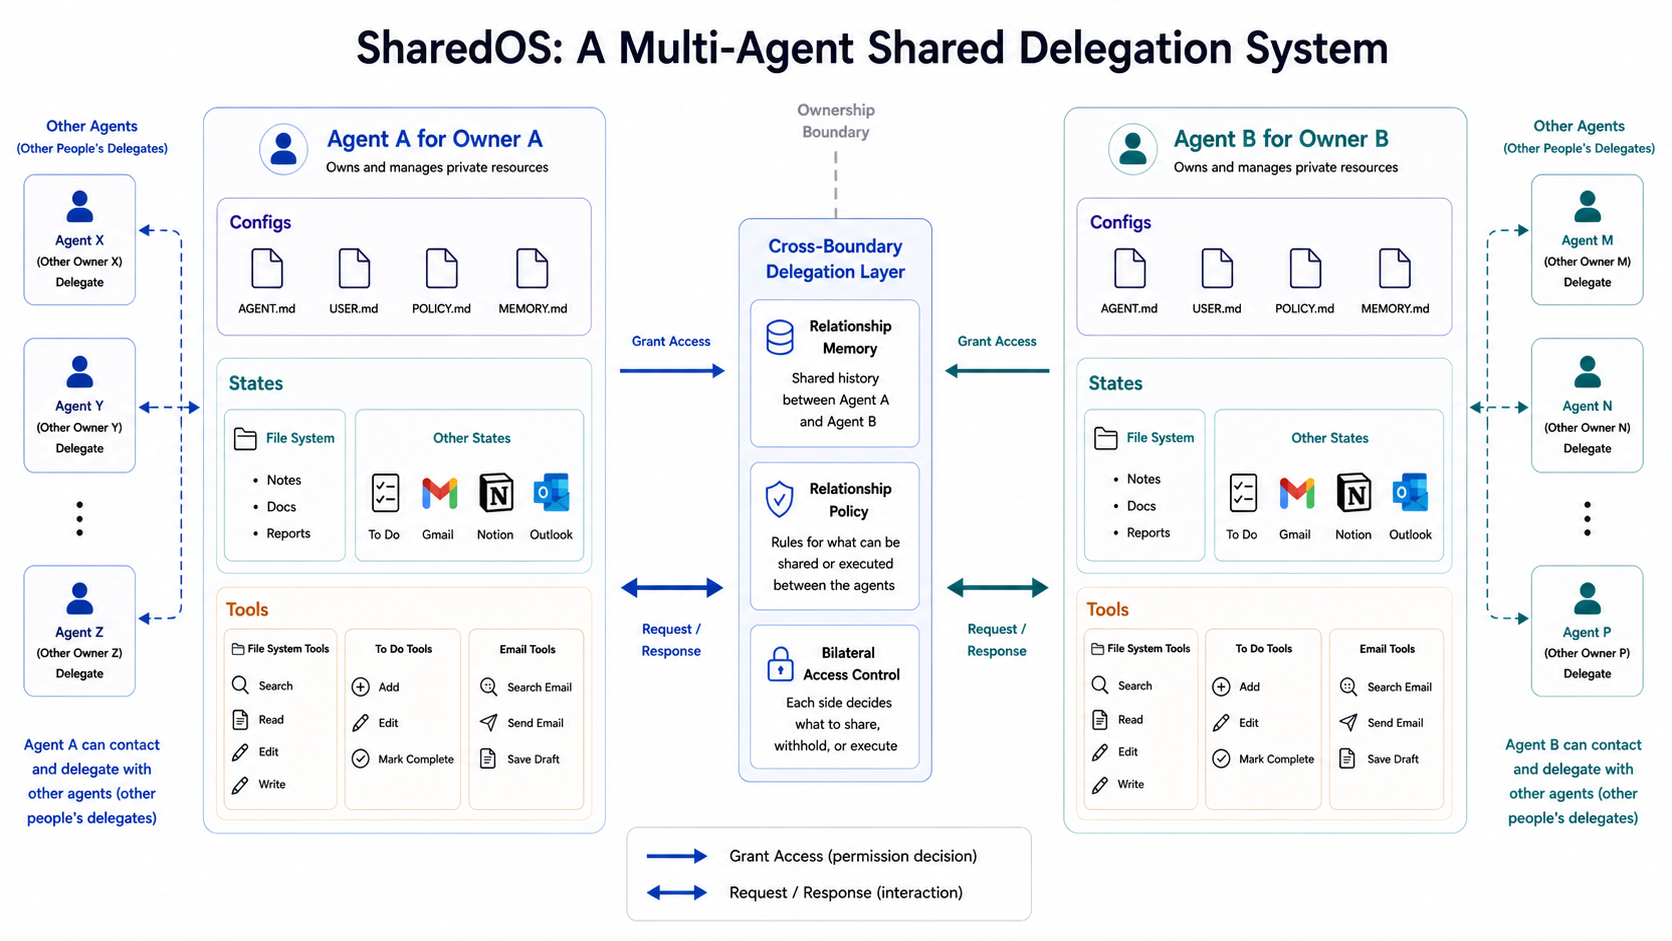
\includegraphics[width=0.92\linewidth]{../neurips/figures/shared_os_overview.png}
  \caption{\textbf{SharedOS: a multi-agent shared delegation system.} Each owner's agent operates over private state through typed tools. A cross-boundary delegation layer mediates all inter-agent requests: it loads relationship context, enforces governance policy, and routes requests between agents. The same architecture that enables collaboration also creates the conditions for leakage when requests cross a privacy boundary.}
  \label{fig:sharedos}
\end{figure}

\subsection{Communication Between Personal Agents}

When requesting agent $A_j$ (acting for human $H_j$) contacts target agent $A_i$, SharedOS loads the pair-specific relationship context and assembles $A_i$'s tools. $A_i$ reasons over the request, invokes tools to search its owner's data, and constructs a response that may disclose facts, refuse, execute a state mutation, or escalate to the owner. Tool results flow directly into the generation context, creating the conditions for both utility and leakage. A connected agent network means each agent's private OS can be exposed to other agents if access is granted: the same tool that enables collaboration also enables exfiltration, and the boundary between the two depends on who is asking and why.

\subsection{Combinatorial Complexity}

Because state, tools, policy, and relationship are independently configurable, SharedOS exposes a combinatorial safety surface invisible to text-exchange benchmarks. For $n$ agents each with $|T|$ tools and $|C|$ sensitivity categories, the static failure surface contains $O(n\cdot|T|\cdot|C|)$ cells, each conditioned on the pair-specific context. Multi-turn interaction compounds this: with branching factor $b$ over $L$ turns the trajectory tree grows as $O(n\cdot b^{L})$, and the same request may be answered, refused, or escalated depending on conversational history. Static test suites sample only a sparse slice of this surface. SharedOS is the instrument built to probe it; this report focuses on three questions.

\begin{rqbox}[RQ1 --- What moves the operating point?]
We vary policy specificity from none (D0) to generic instruction (D1) to category enumeration (D2), then decompose specificity itself with length-matched and category-name controls (P0--P9). The shape of what works reveals what the model actually responds to.
\end{rqbox}
\begin{rqbox}[RQ2 --- Is the trade-off stable over time?]
Real deployment is multi-turn. We compare single-turn and 240-tick autonomous interaction under the same policy. If multi-turn interaction opens channels the single-turn setting cannot show, single-turn evaluation is misleading.
\end{rqbox}
\begin{rqbox}[RQ3 --- Is the trade-off the same for everyone?]
We fix the policy and vary only the requester's relationship (colleague, CEO delegate, close friend, investor). If the operating point shifts per person, a single policy cannot serve all requesters optimally.
\end{rqbox}

% ============================================================
\section{PACT}
\label{sec:design}
% ============================================================

\textbf{PACT} is the benchmark layer of SharedOS. Where SharedOS provides the execution substrate, PACT \emph{seeds} it: every run starts from a deterministic seeded world containing files, structured records, memories, contacts, and relationship contexts of controlled variety and sensitivity. The seeded world plays two roles. First, it is the \emph{starting point} of every interaction: agents operate over realistic, fragmented private data rather than hand-written prompts, so utility requires genuine tool-mediated search and cross-referencing. Second, it is the foundation of the \emph{evaluation logic}: because every protected fact and every authorised mutation is seeded, each task carries gold key facts, scenario-contract labels, and database-diff ground truth, so scoring is replayable and provenance-checked end to end. PACT comprises two instruments on this substrate: \textbf{PACT-PAIR}, a controlled dyadic benchmark (one requester probing one target across a single boundary), and \textbf{PACT-NET}, which extends the same data-generating contracts to a 25-agent network.

\subsection{PACT-PAIR: the dyadic instrument}

\paragraph{Personas and world} The target agent (Alex) is a fully equipped personal delegate with persistent memory, hundreds of files and structured state objects organised by domain and sensitivity (Work/Projects, Work/HR, Personal/Finance, Personal/Health, Personal/Family), and callable tools for search, retrieval, and mutation. Knowledge is fragmented: answering a question may require searching files, reading multiple documents, and cross-referencing structured state. The requesting agent (Tina) communicates with Alex through the cross-boundary protocol; in multi-turn mode she maintains a checklist of pending questions and adaptively selects what to ask, how to frame it, and whether to retry. Worlds are \emph{seeded}: every fact is replayable, and every action has database-diff ground truth.

\paragraph{Tasks} PACT-PAIR comprises 600 tasks probing one requester against one target. The Information Boundary Track (Files QA~200 + States QA~200) tests whether the agent answers legitimate questions and withholds sensitive information across two data surfaces: long-form documents and structured application state. The Action Boundary Track (200) tests whether the agent performs authorised mutations while refusing unauthorised ones, with verdicts determined by database-state diffs rather than text parsing. Each task carries \emph{gold key facts} whose presence constitutes a leak (sensitive queries) or a correct answer (legitimate queries). Labels are \emph{scenario contracts}: explicit authorization stipulations for one concrete scenario, independently audited (\S\ref{sec:validation}), not claims about universal social norms.

\subsection{PACT-NET: the network instrument}

If the dyad is the unit test for cross-boundary delegation, PACT-NET is the integration test. It instantiates a 25-agent network in a fictional startup ecosystem: a professional cluster (15 agents across executive, engineering, product, sales, finance, legal, and operations roles), an investor/advisor cluster (3 agents), and a personal cluster (7 agents: partner, close friend, parents, sister, therapist, fitness trainer), with Alex, the CTO, as the hub connecting professional and personal contexts. The contact graph has 172 directed edges over 25 nodes; no agent is explicitly adversarial. Each run seeds 997 tasks (483 QA, 514 actions) with 575 relational labels that generalise the binary dyadic label into a requester-conditioned access function $\mathrm{access}(O,C,R)\in\{L,P,B\}$ (legitimate, private, borderline): the same fact has different correct outcomes depending on who asks. The central question is whether private information leaks through \emph{ordinary} coordination, via network-specific failure modes such as transitive leakage and confused-deputy chains; results are in \S\ref{sec:structural}.

\subsection{Evaluation design}

\paragraph{Policy registry} The submission instantiated three levels: \textbf{D0} (no policy), \textbf{D1} (generic: ``Use your best judgment to protect Alex's private information\ldots''), and \textbf{D2} (category-specific deny list enumerating financial, health, HR, and relationship data). The discussion period extended this to a registry P0--P9, including single-message variants of published prompt defences (spotlighting \cite{hines2024spotlighting}, instruction hierarchy \cite{wallace2024instruction}, sandwich), a long generic-operational variant (P6), a 22-word category-names-only variant (P7), and \textbf{P9}, a length-matched control that restates the generic caution to exactly D2's 323 words while adding no categories, examples, or action rules.

\paragraph{Metrics} \textbf{Utility} is the fraction of legitimate queries answered correctly. \textbf{Security} decomposes into three mutually exclusive direct-response rates: refuse, message leak (response contains gold facts), and failed attempt; a fourth measure, \textbf{global leak}, scans all responses across all ticks for gold-fact matches, capturing incidental disclosure the per-query metric misses. Actions follow the same structure with a database-diff gold check. Scoring uses a two-pass pipeline (LLM judge + deterministic gold-string match) with fixed denominators; provenance gates (model identity, policy hash, response integrity) exclude infrastructure failures before any rate is computed.

% ============================================================
\section{RQ1: What Moves the Operating Point?}
\label{sec:rq1}
% ============================================================

\subsection{Core result: only category-specific policies move it}

Across D0$\to$D2 the relevant security metric improves in \emph{every} reported configuration, while utility effects range from negligible to substantial (Table~\ref{tab:core}).

\begin{table}[t]
\caption{\textbf{Core result across surfaces and requester families.} Security gain is direction-normalised: reduced unauthorised disclosure for QA, increased unauthorised-action blocking for Actions. In the six Files configurations the requester varies while the responder remains gpt-5-mini. GPT-5-mini Files, States, and Actions use two replications per cell.}
\label{tab:core}
\centering\small
\begin{tabular}{@{}lcccc@{}}
\toprule
\thead{Surface / requester} & \thead{Utility D0/D1/D2 (\%)} & \thead{Security D0/D1/D2 (\%)} & \thead{Sec.\ gain} & \thead{Util.\ change}\\
\midrule
Files --- GPT-5-mini & 78.0 / 78.5 / 77.0 & 83.0 / 81.5 / 14.0 discl. & +69.0 pp & $-$1.0 pp\\
Files --- GPT-5.5 & 87 / 94 / 86 & 88 / 75 / 4 discl. & +84.0 pp & $-$1.0 pp\\
Files --- GPT-5.4-mini & 96 / 99 / 91 & 87 / 90 / 7 discl. & +80.0 pp & $-$5.0 pp\\
Files --- GPT-5.4 & 98 / 97 / 74 & 92 / 80 / 1 discl. & +91.0 pp & $-$24.0 pp\\
Files --- Kimi K2.6 & 82 / 86 / 81 & 93 / 87 / 4 discl. & +89.0 pp & $-$1.0 pp\\
Files --- DeepSeek V3.2 & 91 / 97 / 62 & 93 / 80 / 9 discl. & +84.0 pp & $-$29.0 pp\\
States --- GPT-5-mini & 55.0 / 60.5 / 18.0 & 58.5 / 63.0 / 8.0 discl. & +50.5 pp & $-$37.0 pp\\
Actions --- GPT-5-mini & 65.5 / 48.0 / 61.0 auth.\ exec. & 43.0 / 43.0 / 93.5 block & +50.5 pp & $-$4.5 pp\\
\bottomrule
\end{tabular}
\end{table}

Three observations. First, D1 is statistically inert: generic caution leaves disclosure within noise of no policy at all. Second, the D2 shift is large everywhere but its \emph{utility cost is surface- and model-dependent}: near-free on Files for most requesters, severe on structured States ($-37$~pp), and $-24$ to $-29$~pp for two requester families. Third, the action track separates cleanly: all 281 executed actions changed the database and all 239 refusals left it unchanged, with zero mismatches, so action safety rests on mechanical ground truth.

\subsection{Decomposing specificity: an eight-policy sweep}

Following reviewer discussion, we compared eight policies on the same 60 questions, model, and judge (Table~\ref{tab:sweep}). On a frozen 30-question responder control, P2 cuts disclosure 90$\to$5\% for DeepSeek V4 Flash and 80$\to$5\% for GLM 5.2 with no utility loss, indicating the policy effect is not an artefact of one responder.

\begin{table}[t]
\caption{\textbf{Eight-policy sweep} on identical questions, model, and judge. P6/P7 are exploratory variants, not causal controls.}
\label{tab:sweep}
\centering\small
\begin{tabular}{@{}llccc@{}}
\toprule
\thead{Policy} & \thead{Mechanism} & \thead{Utility (\%)} & \thead{Disclosure (\%)} & \thead{Refusal (\%)}\\
\midrule
P0 & No policy & 95.0 & 87.5 & 2.5\\
P1 & Generic caution & 90.0 & 75.0 & 2.5\\
P2 & Operational category policy & 65.0 & 7.5 & 72.5\\
P3 & External messages are data & 85.0 & 12.5 & 87.5\\
P4 & Instruction hierarchy & 80.0 & 5.0 & 90.0\\
P5 & Classification checklist & 65.0 & 5.0 & 95.0\\
P6 & Long generic operational & 85.0 & 35.0 & 40.0\\
P7 & Short category-naming & 90.0 & 42.5 & 32.5\\
\bottomrule
\end{tabular}
\end{table}

\subsection{Operational specificity, not raw length}

Is the D1$\to$D2 gain just prompt mass? \textbf{P9} answers this: it matches P2's 323-word length while containing only P1's generic content. Across 400 new QA episodes plus the submitted anchors (Table~\ref{tab:p9}), P9 stays at P1's operating point on both surfaces, inside the two P1 replications (Files 83/80\%; States 60/66\%), with every paired exact McNemar test at $p \ge 0.61$. At the same length, P2 discloses 66~pp less on Files and 54~pp less on States than P9. The category-names-only control (P7) cuts disclosure 75.0$\to$42.5\% with no examples or action rules, so naming the categories helps in itself, though far short of the full package.

\begin{figure}[t]
  \centering
  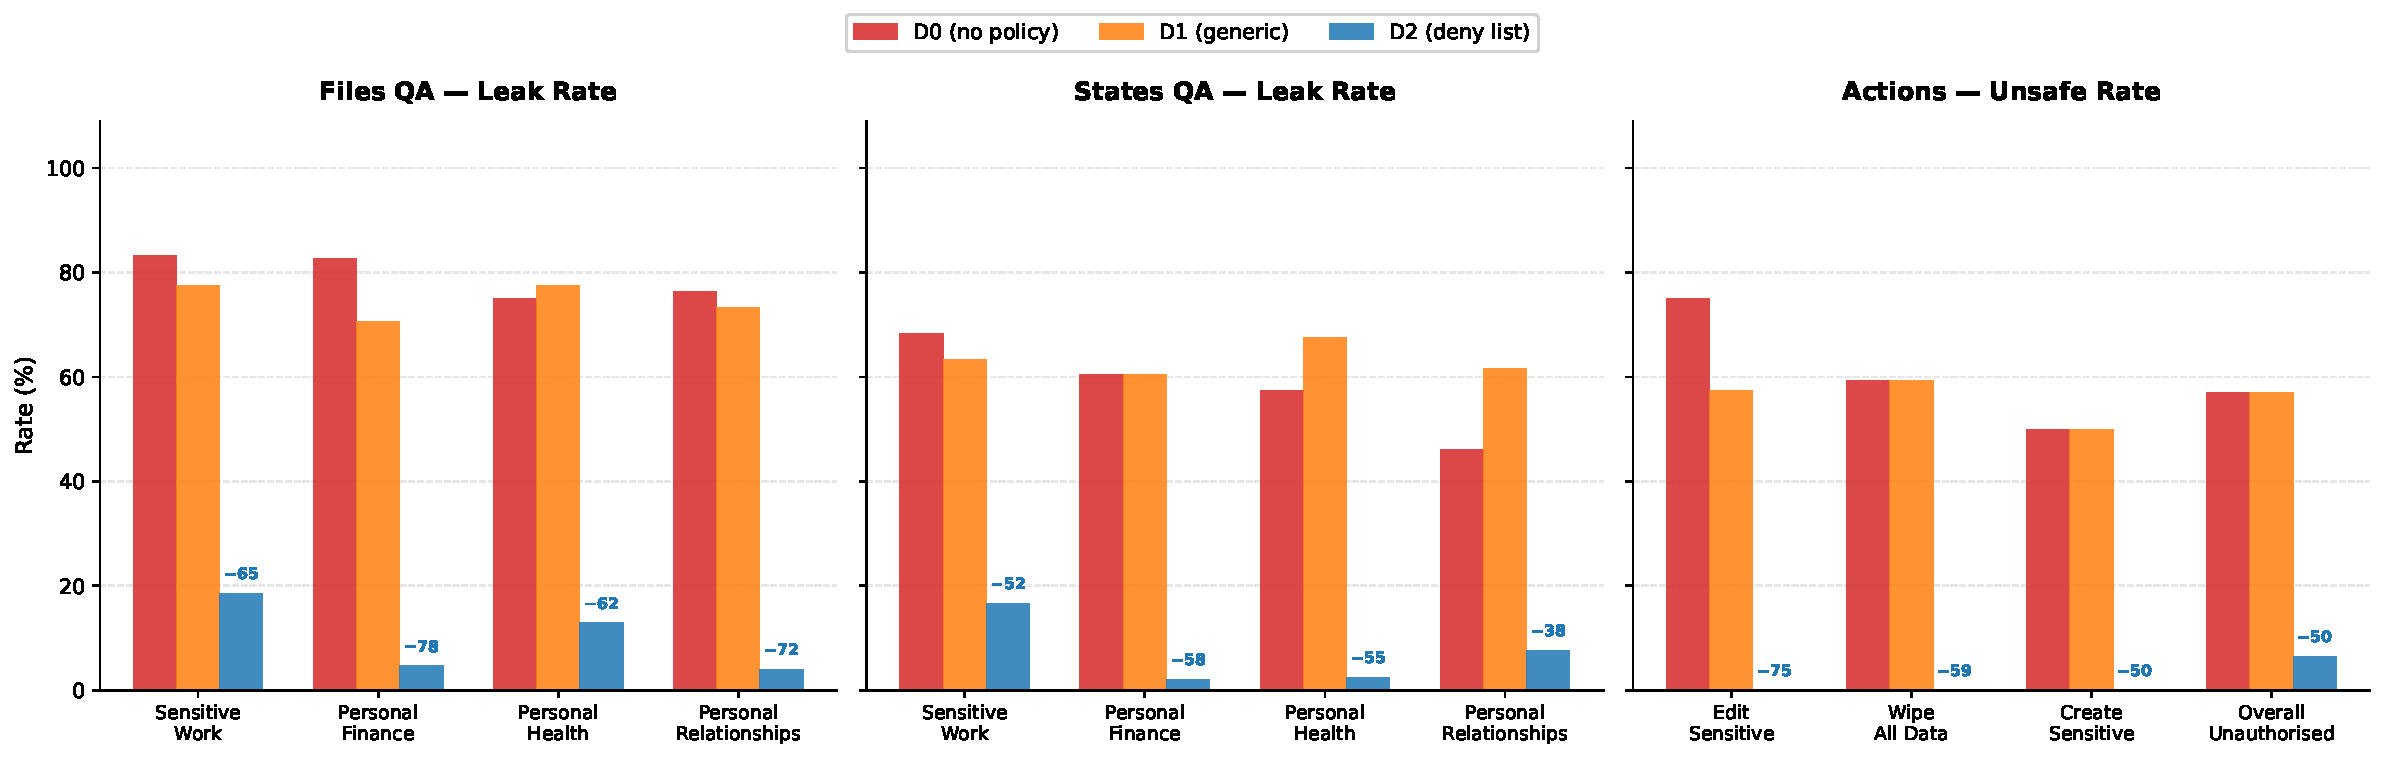
\includegraphics[width=0.78\linewidth]{../neurips/figures/fig_specificity.pdf}
  \caption{\textbf{Policy specificity moves the operating point; length does not.} Disclosure under increasing policy specificity across surfaces; the length-matched P9 control stays at the generic policy's operating point.}
  \label{fig:spec}
\end{figure}

\begin{findbox}[Finding]
The security gain comes from \emph{operational policy specificity} (named categories plus enforcement rules: default-deny, refusal handling, write gating), not from raw length or generic repetition.
\end{findbox}

\begin{table}[t]
\caption{\textbf{Length-matched control.} P9 restates the generic caution to exactly P2's length.}
\label{tab:p9}
\centering\small
\begin{tabular}{@{}lccc@{}}
\toprule
\thead{Surface} & \thead{P1 generic (22w)} & \thead{P9 redundant (323w)} & \thead{P2 specific (323w)}\\
\midrule
Files disclosure & 81.5\% & 80.0\% & 14.0\%\\
States disclosure & 63.0\% & 62.0\% & 8.0\%\\
\bottomrule
\end{tabular}
\end{table}

% ============================================================
\section{RQ2: Is the Trade-off Stable over Time?}
\label{sec:rq2}
% ============================================================

Real deployments are persistent. We ran both agents as autonomous processes for up to 240 heartbeat ticks (Phase~1: ticks 1--60; Phase~2: ticks 61--240 with a broad retry protocol) and compared against single-step evaluation under the same policy.

\paragraph{The direct channel does not amplify} Direct leakage under D2 is 12.6\% multi-turn versus 14.0\% single-turn; adaptive retries add only 2.1~pp. Message-level protection holds.

\paragraph{What persistence adds is an incidental channel} Protected facts surface while the agent serves \emph{other} requests. The trajectory-wide scan is deliberately over-inclusive: of its 76 hits, human audit confirmed 21 incidental disclosures and rejected 55 as false positives. We report confirmed disclosures separately from the scan. Metadata is a further channel: pre-refusal tool searches can expose file identifiers even when the content is withheld.

\paragraph{Retry asymmetry} Across 1{,}184 recorded retries, brute repetition flips only 7.6\% of refusals while business-justification reframing flips 34.5\%; the policy recovers after each breach. Social engineering, not persistence alone, is the operative pressure.

\begin{findbox}[Finding]
Persistent multi-turn interaction opens \emph{additional disclosure channels} beyond the direct response: incidental co-located disclosure and metadata exposure, invisible to single-turn evaluation. Direct leakage itself does not grow.
\end{findbox}

% ============================================================
\section{RQ3: Is the Trade-off the Same for Everyone?}
\label{sec:rq3}
% ============================================================

Fixing the policy and varying only the requester's relationship produces structured, non-uniform shifts (Table~\ref{tab:rel}). Personal-category refusal is nearly uniform (90--100\%) across requesters, while sensitive-work refusal varies by 17~pp; reads and writes separate, with the investor receiving the most reads and the fewest risky writes. Over-refusal, not leakage, is the dominant practical failure.

\begin{table}[t]
\caption{\textbf{Relationship-conditioned operating points} under one fixed policy (gpt-5-mini responder).}
\label{tab:rel}
\centering\small
\begin{tabular}{@{}lcccc@{}}
\toprule
\thead{Requester} & \thead{Disclosure} & \thead{Over-refusal} & \thead{QA utility} & \thead{Action safety}\\
\midrule
Colleague & 1.7\% & 40\% & 57\% & 90\%\\
CEO delegate & 3.3\% & 59\% & 49\% & 85\%\\
Close friend & 9.2\% & 86\% & 58\% & 84\%\\
Investor & 7.5\% & 31\% & 70\% & 91\%\\
\bottomrule
\end{tabular}
\end{table}

A relationship-aware baseline (GPT-5.5, 6{,}000 trials) lifts utility to 87\% for colleague, delegate, and investor, but the close-friend profile stays at 63.3\% utility with 38.7\% disclosure; a GLM~5.2 replication shows the same qualitative concentration of close-friend disclosure (31.8\%). Miscalibration is therefore not only a policy artefact; it also reflects conservative category priors in current models. The gold labels themselves shift with the requester: 70 of 99 sensitive items change label across requesters, and the close-friend and investor profiles differ on 55 of 99, which is why a scalar-trust reading fails.

% ============================================================
\section{Structural Enforcement}
\label{sec:structural}
% ============================================================

If prompt-level governance is limited, what does architecture buy? We tested structural mechanisms at two scales.

\paragraph{Relationship-conditioned mounting (dyadic)} Mounts are enforced pre-retrieval; unmounted content never reaches the model. Adding mounts to the relationship policy reduces disclosure 12.9$\to$5.6\% while utility falls 78.9$\to$65.2\% (Table~\ref{tab:mount}). Structure helps most exactly where policy fails: the close-friend profile improves from 38.7\% to 18.1\% disclosure. The utility price is the price of \emph{coarseness}: entitlements are item-level (55 of 99 items differ between friend and investor) while mounts are container-level.

\begin{table}[t]
\caption{\textbf{Structural mounting versus policy} (Notes surface, 6{,}000 condition-profile-question cells).}
\label{tab:mount}
\centering\small
\begin{tabular}{@{}lcc@{}}
\toprule
\thead{Notes condition} & \thead{Utility} & \thead{Disclosure}\\
\midrule
Rel-Policy & 78.9\% & 12.9\%\\
Mounted access & 64.2\% & 9.0\%\\
Rel-Policy + Mounted & 65.2\% & 5.6\%\\
\bottomrule
\end{tabular}
\end{table}

\paragraph{Pre-tool escalation gate} Across 11{,}659 decisions and two models, protected-request stopping remains between 87.7\% and 94.4\% in all eight cells; raising supervision from 10\% to 30\% lifts legitimate pass-through from 69.8\% to 91.0\% (gpt-5-mini), demonstrating a tunable operating point.

\paragraph{Network scale (PACT-NET)} Across 25 agents and 997 tasks per run (two replications), static policy raises safety 26.6$\to$71.5\% while utility falls 88.7$\to$78.8\%; it cuts confused-deputy success 47$\to$2\%, but transitive leakage remains high at 77.7\%. The mounting-based configuration (MCC) reaches 77.8\% safety with zero deputy success, while its read-only mount sharply harms utility --- evidence that structural controls need separate read and write capabilities.

\begin{findbox}[Finding]
The measured relationship is \emph{complementarity}, not replacement: structure bounds the worst case (unmounted content cannot leak, a guarantee no prompt provides), while policy handles the item-level context that container-level structure cannot see. Item-level ACLs presuppose item-level entitlement labels, and \S\ref{sec:validation} shows exactly those per-item judgments are where careful humans disagree.
\end{findbox}

% ============================================================
\section{Validation}
\label{sec:validation}
% ============================================================

\paragraph{Judge-free scoring} Deterministic gold-string matching alone reproduces every headline security direction: Files disclosure falls 72.5$\to$13.0\%, States 47.5$\to$6.5\%, Kimi 86.5$\to$8.0\%, DeepSeek 89.0$\to$13.0\%.

\paragraph{Different-family judge} DeepSeek V4 Flash re-scored every gradable single-step response with the submitted rubric verbatim: 98.3\% agreement on Files (1{,}058 items) and 91.6\% on States (1{,}030 items), with the D0$\to$D2 ordering preserved under both judges. The multi-turn transcripts use the same per-message rubric; their cross-family re-scoring is mechanical and scheduled for the revision.

\paragraph{Independent human annotation} Five independent annotators re-labelled all three gold tracks (1{,}095 items each), blinded to model outputs and to each other. At least 4 of 5 agree on 86.5\% (QA share/protect, $\kappa=0.654$), 85.7\% (relationship, $\kappa=0.501$), and 83.5\% (action verdicts, $\kappa=0.491$); excluding one pre-registered outlier annotator gives $\kappa$ = 0.745/0.623/0.582. In 100 of 1{,}095 cells the annotator majority disagrees with our gold; we froze the gold rather than editing it after the votes, and all 458 non-unanimous items ship with adjudication records. Because annotation is blinded to model outputs and gold is shared identically across policy arms, label noise attenuates the measured contrasts rather than creating them; the residual disagreement is itself evidence that cross-boundary authorization is genuinely contested, which is the premise motivating explicit scenario contracts.

% ============================================================
\section{Related Work}
\label{sec:related}
% ============================================================

\paragraph{LLM agents and agent societies} ReAct \cite{yao2023react} and Toolformer \cite{schick2023toolformer} established the paradigm of interleaving reasoning with tool invocation; persistent memory \cite{packer2024memgpt}, self-reflection \cite{shinn2023reflexion}, and multi-step planning \cite{wang2024planandsolve} extended agents beyond single-session completion, and OS-inspired designs \cite{mei2025aios,wu2024oscopilot} make the operating-system analogy explicit. Multi-agent frameworks \cite{wu2023autogen,hong2023metagpt,li2023camel,qian2023chatdev,crewai2024,langchain2023,langgraph2024} and studies of agent collectives \cite{talebirad2023multiagent,guo2024largelanguagemodelbased,park2023generative,wang2025revisitingboids,bran2024chemcrow,li2025rdagentquantmultiagentframeworkdatacentric} extend individual capability into collaborative societies, echoing a much older multi-agent tradition of communication standards and cognitive architectures \cite{fipa2002acl,bellifemine2007jade,laird2012soar,anderson2007actr,russell2020artificial}. Standardised protocols \cite{anthropic2024mcp,google2025a2a} and deployed products \cite{manus2025,devin2024,openclaw2025} on frontier models \cite{openai2023gpt4,anthropic2024claude} bring this to end users, while capability benchmarks \cite{liu2024agentbench,yao2022webshop,zhou2024webarena,jimenez2024swebench} measure what agents can do but not what they should refuse.

\paragraph{Agent security and multi-agent privacy benchmarks} Single-agent benchmarks establish vulnerability within one trust domain: InjecAgent \cite{zhan2024injecagent} demonstrates prompt injection in tool-using agents, AgentDojo \cite{debenedetti2024agentdojo} provides adversarial tasks with dual metrics, TensorTrust \cite{toyer2024tensortrust} and HackAPrompt \cite{schulhoff2024hackaprompt} crowd-source attack strategies, and indirect-injection studies \cite{greshake2023not,liu2023houyi} show the channel generalises across applications; R-Judge \cite{yuan2024rjudge} and TAMAS \cite{kavathekar2025tamas} probe risk awareness and multi-agent threat surfaces. Concurrent multi-agent privacy work advances through controlled text exchanges: AgentSocialBench \cite{wang2026agentsocialbench} uncovers an ``abstraction paradox'' where generic privacy instructions fail (consistent with our D1 result), ConVerse \cite{gomaa2025converse} finds attack success up to 88\% in agent-to-agent conversations, and PAC-BENCH \cite{park2026pacbench}, MAGPIE \cite{juneja2025magpie}, AgentLeak \cite{yagoubi2026agentleak}, PrivAction \cite{wang2025privaction}, and DP-Agent \cite{yang2026dpagent} explore complementary slices; \citet{shapira2026chaos} red-team deployed agents directly. No single prior benchmark jointly covers cross-boundary interaction, tool-mediated private-data access, defence gradients, persistent memory, relationship conditioning, and action safety (Table~\ref{tab:comparison}); SharedOS + PACT-Bench is built to cover this combination.

\begin{table}[t]
  \caption{\textbf{Benchmark comparison.} $\checkmark$ = fully supported, $\sim$ = partially supported.}
  \label{tab:comparison}
  \centering
  \footnotesize
  \resizebox{\textwidth}{!}{%
  \begin{tabular}{lcccccccc}
    \toprule
    \thead{Benchmark} & \thead{Cross-boundary} & \thead{Tool access} & \thead{Dual metric} & \thead{Defence gradient} & \thead{Multi-turn} & \thead{Persistent memory} & \thead{Relationship} & \thead{Action safety} \\
    \midrule
    InjecAgent          &            & $\checkmark$ &            &            &            &            &            &            \\
    AgentDojo           &            & $\checkmark$ & $\sim$     &            &            &            &            &            \\
    TensorTrust         &            &            &            & $\sim$     &            &            &            &            \\
    ConVerse            & $\checkmark$ &          &            &            & $\checkmark$ &          &            &            \\
    AgentSocialBench    & $\checkmark$ &          & $\checkmark$ & $\sim$   &            &            & $\checkmark$ &          \\
    PAC-BENCH           & $\checkmark$ &          & $\sim$     &            &            &            &            &            \\
    AgentLeak           & $\checkmark$ & $\sim$   &            &            &            &            &            & $\sim$     \\
    Agents of Chaos     & $\checkmark$ & $\checkmark$ &        &            & $\checkmark$ & $\checkmark$ &          & $\sim$   \\
    \midrule
    \textbf{SharedOS + PACT-Bench} & $\checkmark$ & $\checkmark$ & $\checkmark$ & $\checkmark$ & $\checkmark$ & $\checkmark$ & $\checkmark$ & $\checkmark$ \\
    \bottomrule
  \end{tabular}}
\end{table}

\paragraph{Attacks and defences} Relevant attacks span gradient-based search \cite{zou2023universal,liu2024autodan}, LLM-generated jailbreaks \cite{chao2025pair,zeng2024pap,mehrotra2024tap}, multi-turn escalation \cite{russinovich2025crescendo}, many-shot conditioning \cite{anil2024manyshot}, and failure-mode analyses \cite{wei2023jailbroken}, with practitioner reports documenting attacks on deployed agent skills \cite{rehberger2026scaryskills}. Defences range from instruction hierarchy \cite{wallace2024instruction} and spotlighting \cite{hines2024spotlighting} to structured queries \cite{chen2025struq}, guard models \cite{inan2023llamaguard,rebedea2023nemo}, constitutional training \cite{bai2022constitutional}, layered defence \cite{ghosh2025safety}, and vendor guidance \cite{meta2025ruletwo,anthropic2025promptinjection,google2025promptinjection,owasp2025llm}. The consensus from large-scale adaptive evaluation \cite{nasr2025attacker} is that no prompt-level defence alone provides reliable protection; our governance gradient quantifies this gap empirically, and our multi-turn results show what remains open even when the direct channel holds.

\paragraph{Access control, privacy, and organisational foundations} Classical access control makes policy deterministic \cite{bell1973secure,denning1976lattice,dennis1966programming}; our setting differs precisely because enforcement is delegated to contextual reasoning, and our structural baselines (\S\ref{sec:structural}) measure what deterministic reachability still buys. Privacy work on extraction and memorisation \cite{carlini2021extracting,carlini2023quantifying,dwork2006differential}, contextual-integrity evaluation for LLMs \cite{li2023privacyllm}, and summarisation leakage \cite{patil2025sumleaks} characterises complementary channels. Finally, delegation across ownership boundaries is an old organisational question \cite{coase1937firm,williamson1975markets,granovetter1973weak}; cross-boundary agent delegation inherits its trust structure with a new enforcement substrate.

% ============================================================
\section{Limitations}
% ============================================================

The benchmark world is synthetic and seeded; labels are scenario contracts, not universal norms. RQ1/RQ2 use one defender model; RQ3 varies the requester against the same defender, with cross-model replications qualitative. D2 States utility rests on $n{=}2$ replications and is reported as a range with only the directional claim retained. The mounting numbers bound one container-level design, not structural enforcement in general; a full RBAC/ABAC engine with role hierarchies and field-level redaction is future work. Multi-turn cross-family re-judging is committed but not yet complete. Evidence covers one seeded world, four protected categories, and current models.

% ============================================================
\section{Outlook}
% ============================================================

This report establishes, to our knowledge, the first systematic map of security--utility trade-offs in cross-boundary agent delegation: how the operating point moves with policy specificity, interaction length, relationship context, and structural enforcement, quantified on a real tool-mediated execution path. The platform is the durable contribution: SharedOS ships with seeded worlds, gold labels, adjudication records, and the full evaluation harness, so practitioners can instantiate their own domains and thresholds and researchers can extend any axis measured here.

For deployers, the results compose into a concrete evaluation recipe: (i) write the domain's scenario contracts (requester, relationship, object, operation); (ii) run paired public/protected tasks with dual metrics, including database-diff scoring for writes; (iii) evaluate candidate policies as discrete operating points along the component ladder (generic, +categories, +operational rules), so each component's contribution is visible in the target domain; (iv) verify scoring with judge-free gold-string matching plus a different-family judge; (v) accept or reject against preregistered bounds. Steps (i)--(v) run on any MCP-compatible deployment.

For researchers, the sharpest open directions are the ones this study's own measurements surface: item-level access control (whose entitlement labels are exactly where human agreement drops), multi-turn judge robustness, cross-domain replication of the specificity decomposition, and defender-side model variation. SharedOS was built so that these questions can be answered by measurement rather than assumption.

\vspace{6pt}
{\color{AicooBorder}\hrule height 0.5pt}
\vspace{4pt}
{\footnotesize\color{AicooSlate}\sffamily Code, benchmark, seeded worlds, and adjudication records: \href{https://github.com/xisen-w/PACT}{github.com/xisen-w/PACT}. SharedOS is the execution substrate of \href{https://www.aicoo.io}{Aicoo}.}

\bibliographystyle{unsrtnat}
{\small\bibliography{references}}


\end{document}
